\documentclass[1p]{elsarticle_modified}
%\bibliographystyle{elsarticle-num}

%\usepackage[colorlinks]{hyperref}
%\usepackage{abbrmath_seonhwa} %\Abb, \Ascr, \Acal ,\Abf, \Afrak
\usepackage{amsfonts}
\usepackage{amssymb}
\usepackage{amsmath}
\usepackage{amsthm}
\usepackage{scalefnt}
\usepackage{amsbsy}
\usepackage{kotex}
\usepackage{caption}
\usepackage{subfig}
\usepackage{color}
\usepackage{graphicx}
\usepackage{xcolor} %% white, black, red, green, blue, cyan, magenta, yellow
\usepackage{float}
\usepackage{setspace}
\usepackage{hyperref}

\usepackage{tikz}
\usetikzlibrary{arrows}

\usepackage{multirow}
\usepackage{array} % fixed length table
\usepackage{hhline}

%%%%%%%%%%%%%%%%%%%%%
\makeatletter
\renewcommand*\env@matrix[1][\arraystretch]{%
	\edef\arraystretch{#1}%
	\hskip -\arraycolsep
	\let\@ifnextchar\new@ifnextchar
	\array{*\c@MaxMatrixCols c}}
\makeatother %https://tex.stackexchange.com/questions/14071/how-can-i-increase-the-line-spacing-in-a-matrix
%%%%%%%%%%%%%%%

\usepackage[normalem]{ulem}

\newcommand{\msout}[1]{\ifmmode\text{\sout{\ensuremath{#1}}}\else\sout{#1}\fi}
%SOURCE: \msout is \stkout macro in https://tex.stackexchange.com/questions/20609/strikeout-in-math-mode

\newcommand{\cancel}[1]{
	\ifmmode
	{\color{red}\msout{#1}}
	\else
	{\color{red}\sout{#1}}
	\fi
}

\newcommand{\add}[1]{
	{\color{blue}\uwave{#1}}
}

\newcommand{\replace}[2]{
	\ifmmode
	{\color{red}\msout{#1}}{\color{blue}\uwave{#2}}
	\else
	{\color{red}\sout{#1}}{\color{blue}\uwave{#2}}
	\fi
}

\newcommand{\Sol}{\mathcal{S}} %segment
\newcommand{\D}{D} %diagram
\newcommand{\A}{\mathcal{A}} %arc


%%%%%%%%%%%%%%%%%%%%%%%%%%%%%5 test

\def\sl{\operatorname{\textup{SL}}(2,\Cbb)}
\def\psl{\operatorname{\textup{PSL}}(2,\Cbb)}
\def\quan{\mkern 1mu \triangleright \mkern 1mu}

\theoremstyle{definition}
\newtheorem{thm}{Theorem}[section]
\newtheorem{prop}[thm]{Proposition}
\newtheorem{lem}[thm]{Lemma}
\newtheorem{ques}[thm]{Question}
\newtheorem{cor}[thm]{Corollary}
\newtheorem{defn}[thm]{Definition}
\newtheorem{exam}[thm]{Example}
\newtheorem{rmk}[thm]{Remark}
\newtheorem{alg}[thm]{Algorithm}

\newcommand{\I}{\sqrt{-1}}
\begin{document}

%\begin{frontmatter}
%
%\title{Boundary parabolic representations of knots up to 8 crossings}
%
%%% Group authors per affiliation:
%\author{Yunhi Cho} 
%\address{Department of Mathematics, University of Seoul, Seoul, Korea}
%\ead{yhcho@uos.ac.kr}
%
%
%\author{Seonhwa Kim} %\fnref{s_kim}}
%\address{Center for Geometry and Physics, Institute for Basic Science, Pohang, 37673, Korea}
%\ead{ryeona17@ibs.re.kr}
%
%\author{Hyuk Kim}
%\address{Department of Mathematical Sciences, Seoul National University, Seoul 08826, Korea}
%\ead{hyukkim@snu.ac.kr}
%
%\author{Seokbeom Yoon}
%\address{Department of Mathematical Sciences, Seoul National University, Seoul, 08826,  Korea}
%\ead{sbyoon15@snu.ac.kr}
%
%\begin{abstract}
%We find all boundary parabolic representation of knots up to 8 crossings.
%
%\end{abstract}
%\begin{keyword}
%    \MSC[2010] 57M25 
%\end{keyword}
%
%\end{frontmatter}

%\linenumbers
%\tableofcontents
%
\newcommand\colored[1]{\textcolor{white}{\rule[-0.35ex]{0.8em}{1.4ex}}\kern-0.8em\color{red} #1}%
%\newcommand\colored[1]{\textcolor{white}{ #1}\kern-2.17ex	\textcolor{white}{ #1}\kern-1.81ex	\textcolor{white}{ #1}\kern-2.15ex\color{red}#1	}

{\Large $\underline{12n_{0161}~(K12n_{0161})}$}

\setlength{\tabcolsep}{10pt}
\renewcommand{\arraystretch}{1.6}
\vspace{1cm}\begin{tabular}{m{100pt}>{\centering\arraybackslash}m{274pt}}
\multirow{5}{120pt}{
	\centering
	\includegraphics[width=112pt]{../../../GIT/diagram.site/Diagrams/png/2250_12n_0161.png}\\
\ \ \ A knot diagram\footnotemark}&
\allowdisplaybreaks
\textbf{Linearized knot diagam} \\
\cline{2-2}
 &
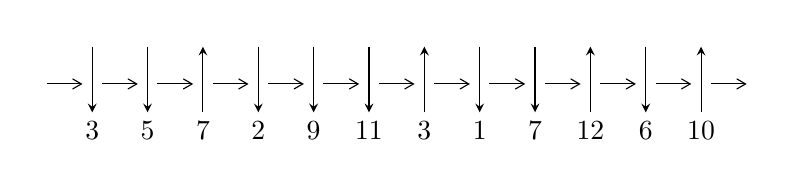
\begin{tikzpicture}[x=20pt, y=17pt]
	% nodes
	\node (C0) at (0, 0) {};
	\node (C1) at (1, 0) {};
	\node (C1U) at (1, +1) {};
	\node (C1D) at (1, -1) {3};

	\node (C2) at (2, 0) {};
	\node (C2U) at (2, +1) {};
	\node (C2D) at (2, -1) {5};

	\node (C3) at (3, 0) {};
	\node (C3U) at (3, +1) {};
	\node (C3D) at (3, -1) {7};

	\node (C4) at (4, 0) {};
	\node (C4U) at (4, +1) {};
	\node (C4D) at (4, -1) {2};

	\node (C5) at (5, 0) {};
	\node (C5U) at (5, +1) {};
	\node (C5D) at (5, -1) {9};

	\node (C6) at (6, 0) {};
	\node (C6U) at (6, +1) {};
	\node (C6D) at (6, -1) {11};

	\node (C7) at (7, 0) {};
	\node (C7U) at (7, +1) {};
	\node (C7D) at (7, -1) {3};

	\node (C8) at (8, 0) {};
	\node (C8U) at (8, +1) {};
	\node (C8D) at (8, -1) {1};

	\node (C9) at (9, 0) {};
	\node (C9U) at (9, +1) {};
	\node (C9D) at (9, -1) {7};

	\node (C10) at (10, 0) {};
	\node (C10U) at (10, +1) {};
	\node (C10D) at (10, -1) {12};

	\node (C11) at (11, 0) {};
	\node (C11U) at (11, +1) {};
	\node (C11D) at (11, -1) {6};

	\node (C12) at (12, 0) {};
	\node (C12U) at (12, +1) {};
	\node (C12D) at (12, -1) {10};
	\node (C13) at (13, 0) {};

	% arrows
	\draw[->,>={angle 60}]
	(C0) edge (C1) (C1) edge (C2) (C2) edge (C3) (C3) edge (C4) (C4) edge (C5) (C5) edge (C6) (C6) edge (C7) (C7) edge (C8) (C8) edge (C9) (C9) edge (C10) (C10) edge (C11) (C11) edge (C12) (C12) edge (C13) ;	\draw[->,>=stealth]
	(C1U) edge (C1D) (C2U) edge (C2D) (C3D) edge (C3U) (C4U) edge (C4D) (C5U) edge (C5D) (C6U) edge (C6D) (C7D) edge (C7U) (C8U) edge (C8D) (C9U) edge (C9D) (C10D) edge (C10U) (C11U) edge (C11D) (C12D) edge (C12U) ;
	\end{tikzpicture} \\
\hhline{~~} \\& 
\textbf{Solving Sequence} \\ \cline{2-2} 
 &
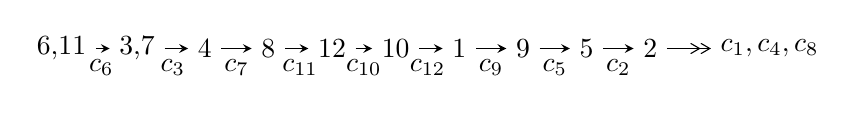
\begin{tikzpicture}[x=23pt, y=7pt]
	% node
	\node (A0) at (-1/8, 0) {6,11};
	\node (A1) at (17/16, 0) {3,7};
	\node (A2) at (17/8, 0) {4};
	\node (A3) at (25/8, 0) {8};
	\node (A4) at (33/8, 0) {12};
	\node (A5) at (41/8, 0) {10};
	\node (A6) at (49/8, 0) {1};
	\node (A7) at (57/8, 0) {9};
	\node (A8) at (65/8, 0) {5};
	\node (A9) at (73/8, 0) {2};
	\node (C1) at (1/2, -1) {$c_{6}$};
	\node (C2) at (13/8, -1) {$c_{3}$};
	\node (C3) at (21/8, -1) {$c_{7}$};
	\node (C4) at (29/8, -1) {$c_{11}$};
	\node (C5) at (37/8, -1) {$c_{10}$};
	\node (C6) at (45/8, -1) {$c_{12}$};
	\node (C7) at (53/8, -1) {$c_{9}$};
	\node (C8) at (61/8, -1) {$c_{5}$};
	\node (C9) at (69/8, -1) {$c_{2}$};
	\node (A10) at (11, 0) {$c_{1},c_{4},c_{8}$};

	% edge
	\draw[->,>=stealth]	
	(A0) edge (A1) (A1) edge (A2) (A2) edge (A3) (A3) edge (A4) (A4) edge (A5) (A5) edge (A6) (A6) edge (A7) (A7) edge (A8) (A8) edge (A9) ;
	\draw[->>,>={angle 60}]	
	(A9) edge (A10);
\end{tikzpicture} \\ 

\end{tabular} \\

\footnotetext{
The image of knot diagram is generated by the software ``\textbf{Draw programme}" developed by Andrew Bartholomew(\url{http://www.layer8.co.uk/maths/draw/index.htm\#Running-draw}), where we modified some parts for our purpose(\url{https://github.com/CATsTAILs/LinksPainter}).
}\phantom \\ \newline 
\centering \textbf{Ideals for irreducible components\footnotemark of $X_{\text{par}}$} 
 
\begin{align*}
I^u_{1}&=\langle 
- u^{52}+u^{51}+\cdots+b+u,\;- u^{52}+u^{51}+\cdots+a+5 u,\;u^{54}-2 u^{53}+\cdots+4 u^2-1\rangle \\
I^u_{2}&=\langle 
- u^5- u^3+b- u+1,\;u^7+u^6+2 u^5+u^4+2 u^3+u^2+a+u,\;u^9+u^8+2 u^7+u^6+3 u^5+u^4+2 u^3+u-1\rangle \\
\\
\end{align*}
\raggedright * 2 irreducible components of $\dim_{\mathbb{C}}=0$, with total 63 representations.\\
\footnotetext{All coefficients of polynomials are rational numbers. But the coefficients are sometimes approximated in decimal forms when there is not enough margin.}
\newpage
\renewcommand{\arraystretch}{1}
\centering \section*{I. $I^u_{1}= \langle - u^{52}+u^{51}+\cdots+b+u,\;- u^{52}+u^{51}+\cdots+a+5 u,\;u^{54}-2 u^{53}+\cdots+4 u^2-1 \rangle$}
\flushleft \textbf{(i) Arc colorings}\\
\begin{tabular}{m{7pt} m{180pt} m{7pt} m{180pt} }
\flushright $a_{6}=$&$\begin{pmatrix}1\\0\end{pmatrix}$ \\
\flushright $a_{11}=$&$\begin{pmatrix}0\\u\end{pmatrix}$ \\
\flushright $a_{3}=$&$\begin{pmatrix}u^{52}- u^{51}+\cdots+6 u^2-5 u\\u^{52}- u^{51}+\cdots+3 u^2- u\end{pmatrix}$ \\
\flushright $a_{7}=$&$\begin{pmatrix}1\\u^2\end{pmatrix}$ \\
\flushright $a_{4}=$&$\begin{pmatrix}- u^{53}+3 u^{52}+\cdots-6 u-1\\u^{53}+u^{52}+\cdots+2 u^2-2 u\end{pmatrix}$ \\
\flushright $a_{8}=$&$\begin{pmatrix}u^{17}+2 u^{15}+5 u^{13}+6 u^{11}+7 u^9+6 u^7+4 u^5+2 u^3+u\\- u^{17}-3 u^{15}-7 u^{13}-10 u^{11}-11 u^9-8 u^7-4 u^5+u\end{pmatrix}$ \\
\flushright $a_{12}=$&$\begin{pmatrix}- u\\u\end{pmatrix}$ \\
\flushright $a_{10}=$&$\begin{pmatrix}- u^3\\u^3+u\end{pmatrix}$ \\
\flushright $a_{1}=$&$\begin{pmatrix}- u^5- u\\u^5+u^3+u\end{pmatrix}$ \\
\flushright $a_{9}=$&$\begin{pmatrix}u^5+u\\u^7+u^5+2 u^3+u\end{pmatrix}$ \\
\flushright $a_{5}=$&$\begin{pmatrix}- u^{12}- u^{10}-3 u^8-2 u^6-2 u^4- u^2+1\\- u^{14}-2 u^{12}-5 u^{10}-6 u^8-6 u^6-4 u^4- u^2\end{pmatrix}$ \\
\flushright $a_{2}=$&$\begin{pmatrix}u^{50}- u^{49}+\cdots-5 u+1\\u^{52}- u^{51}+\cdots-5 u^3+3 u^2\end{pmatrix}$\\&\end{tabular}
\flushleft \textbf{(ii) Obstruction class $= -1$}\\~\\
\flushleft \textbf{(iii) Cusp Shapes $= -4 u^{53}+2 u^{52}+\cdots+4 u-2$}\\~\\
\newpage\renewcommand{\arraystretch}{1}
\flushleft \textbf{(iv) u-Polynomials at the component}\newline \\
\begin{tabular}{m{50pt}|m{274pt}}
Crossings & \hspace{64pt}u-Polynomials at each crossing \\
\hline $$\begin{aligned}c_{1}\end{aligned}$$&$\begin{aligned}
&u^{54}+14 u^{53}+\cdots+12 u+1
\end{aligned}$\\
\hline $$\begin{aligned}c_{2},c_{4}\end{aligned}$$&$\begin{aligned}
&u^{54}-10 u^{53}+\cdots+8 u-1
\end{aligned}$\\
\hline $$\begin{aligned}c_{3},c_{7}\end{aligned}$$&$\begin{aligned}
&u^{54}- u^{53}+\cdots-1024 u+512
\end{aligned}$\\
\hline $$\begin{aligned}c_{5}\end{aligned}$$&$\begin{aligned}
&u^{54}+2 u^{53}+\cdots+220 u-200
\end{aligned}$\\
\hline $$\begin{aligned}c_{6},c_{11}\end{aligned}$$&$\begin{aligned}
&u^{54}+2 u^{53}+\cdots+4 u^2-1
\end{aligned}$\\
\hline $$\begin{aligned}c_{8}\end{aligned}$$&$\begin{aligned}
&u^{54}-2 u^{53}+\cdots-2 u+1
\end{aligned}$\\
\hline $$\begin{aligned}c_{9}\end{aligned}$$&$\begin{aligned}
&u^{54}-10 u^{53}+\cdots+676 u-61
\end{aligned}$\\
\hline $$\begin{aligned}c_{10},c_{12}\end{aligned}$$&$\begin{aligned}
&u^{54}-18 u^{53}+\cdots+8 u+1
\end{aligned}$\\
\hline
\end{tabular}\\~\\
\newpage\renewcommand{\arraystretch}{1}
\flushleft \textbf{(v) Riley Polynomials at the component}\newline \\
\begin{tabular}{m{50pt}|m{274pt}}
Crossings & \hspace{64pt}Riley Polynomials at each crossing \\
\hline $$\begin{aligned}c_{1}\end{aligned}$$&$\begin{aligned}
&y^{54}+62 y^{53}+\cdots-72 y+1
\end{aligned}$\\
\hline $$\begin{aligned}c_{2},c_{4}\end{aligned}$$&$\begin{aligned}
&y^{54}-14 y^{53}+\cdots-12 y+1
\end{aligned}$\\
\hline $$\begin{aligned}c_{3},c_{7}\end{aligned}$$&$\begin{aligned}
&y^{54}-57 y^{53}+\cdots-5767168 y+262144
\end{aligned}$\\
\hline $$\begin{aligned}c_{5}\end{aligned}$$&$\begin{aligned}
&y^{54}+2 y^{53}+\cdots+341200 y+40000
\end{aligned}$\\
\hline $$\begin{aligned}c_{6},c_{11}\end{aligned}$$&$\begin{aligned}
&y^{54}+18 y^{53}+\cdots-8 y+1
\end{aligned}$\\
\hline $$\begin{aligned}c_{8}\end{aligned}$$&$\begin{aligned}
&y^{54}+62 y^{53}+\cdots-8 y+1
\end{aligned}$\\
\hline $$\begin{aligned}c_{9}\end{aligned}$$&$\begin{aligned}
&y^{54}+10 y^{53}+\cdots-22900 y+3721
\end{aligned}$\\
\hline $$\begin{aligned}c_{10},c_{12}\end{aligned}$$&$\begin{aligned}
&y^{54}+38 y^{53}+\cdots-68 y+1
\end{aligned}$\\
\hline
\end{tabular}\\~\\
\newpage\flushleft \textbf{(vi) Complex Volumes and Cusp Shapes}
$$\begin{array}{c|c|c}  
\text{Solutions to }I^u_{1}& \I (\text{vol} + \sqrt{-1}CS) & \text{Cusp shape}\\
 \hline 
\begin{aligned}
u &= \phantom{-}0.593814 + 0.806287 I \\
a &= -0.636999 - 0.227987 I \\
b &= -0.1217130 - 0.0332567 I\end{aligned}
 & -0.33427 - 1.89104 I & -1.02934 + 3.26612 I \\ \hline\begin{aligned}
u &= \phantom{-}0.593814 - 0.806287 I \\
a &= -0.636999 + 0.227987 I \\
b &= -0.1217130 + 0.0332567 I\end{aligned}
 & -0.33427 + 1.89104 I & -1.02934 - 3.26612 I \\ \hline\begin{aligned}
u &= \phantom{-}0.180121 + 0.965813 I \\
a &= -0.594859 - 0.700416 I \\
b &= \phantom{-}0.136216 + 0.368678 I\end{aligned}
 & \phantom{-}1.26301 - 2.44603 I & \phantom{-}2.73199 + 4.98223 I \\ \hline\begin{aligned}
u &= \phantom{-}0.180121 - 0.965813 I \\
a &= -0.594859 + 0.700416 I \\
b &= \phantom{-}0.136216 - 0.368678 I\end{aligned}
 & \phantom{-}1.26301 + 2.44603 I & \phantom{-}2.73199 - 4.98223 I \\ \hline\begin{aligned}
u &= \phantom{-}0.071641 + 1.019550 I \\
a &= \phantom{-}1.27503 - 1.16413 I \\
b &= -0.851885 + 0.413364 I\end{aligned}
 & \phantom{-}3.28922 - 2.50118 I & \phantom{-}2.52265 + 4.62453 I \\ \hline\begin{aligned}
u &= \phantom{-}0.071641 - 1.019550 I \\
a &= \phantom{-}1.27503 + 1.16413 I \\
b &= -0.851885 - 0.413364 I\end{aligned}
 & \phantom{-}3.28922 + 2.50118 I & \phantom{-}2.52265 - 4.62453 I \\ \hline\begin{aligned}
u &= -0.760882 + 0.685041 I \\
a &= -0.333764 - 0.729244 I \\
b &= -0.91421 + 1.34330 I\end{aligned}
 & -2.42886 - 2.49711 I & -6.09592 + 3.26971 I \\ \hline\begin{aligned}
u &= -0.760882 - 0.685041 I \\
a &= -0.333764 + 0.729244 I \\
b &= -0.91421 - 1.34330 I\end{aligned}
 & -2.42886 + 2.49711 I & -6.09592 - 3.26971 I \\ \hline\begin{aligned}
u &= \phantom{-}0.803356 + 0.644099 I \\
a &= -0.363676 + 0.484008 I \\
b &= -2.27231 - 0.36526 I\end{aligned}
 & \phantom{-}4.20288 + 1.73783 I & -3.96774 + 0.13211 I \\ \hline\begin{aligned}
u &= \phantom{-}0.803356 - 0.644099 I \\
a &= -0.363676 - 0.484008 I \\
b &= -2.27231 + 0.36526 I\end{aligned}
 & \phantom{-}4.20288 - 1.73783 I & -3.96774 - 0.13211 I\\
 \hline 
 \end{array}$$\newpage$$\begin{array}{c|c|c}  
\text{Solutions to }I^u_{1}& \I (\text{vol} + \sqrt{-1}CS) & \text{Cusp shape}\\
 \hline 
\begin{aligned}
u &= \phantom{-}0.743941 + 0.723947 I \\
a &= \phantom{-}1.296630 + 0.497606 I \\
b &= \phantom{-}0.351768 + 1.145760 I\end{aligned}
 & -4.60943 + 0.53524 I & -6.65010 + 0.78439 I \\ \hline\begin{aligned}
u &= \phantom{-}0.743941 - 0.723947 I \\
a &= \phantom{-}1.296630 - 0.497606 I \\
b &= \phantom{-}0.351768 - 1.145760 I\end{aligned}
 & -4.60943 - 0.53524 I & -6.65010 - 0.78439 I \\ \hline\begin{aligned}
u &= -0.040432 + 0.958127 I \\
a &= -2.37271 + 0.02401 I \\
b &= \phantom{-}1.54595 + 0.64385 I\end{aligned}
 & \phantom{-}0.680231 + 1.026360 I & \phantom{-}0.362891 + 0.577482 I \\ \hline\begin{aligned}
u &= -0.040432 - 0.958127 I \\
a &= -2.37271 - 0.02401 I \\
b &= \phantom{-}1.54595 - 0.64385 I\end{aligned}
 & \phantom{-}0.680231 - 1.026360 I & \phantom{-}0.362891 - 0.577482 I \\ \hline\begin{aligned}
u &= -0.714465 + 0.763494 I \\
a &= \phantom{-}0.138140 + 1.250370 I \\
b &= \phantom{-}1.70446 - 1.06690 I\end{aligned}
 & -3.72278 + 1.64945 I & -9.08237 - 1.96376 I \\ \hline\begin{aligned}
u &= -0.714465 - 0.763494 I \\
a &= \phantom{-}0.138140 - 1.250370 I \\
b &= \phantom{-}1.70446 + 1.06690 I\end{aligned}
 & -3.72278 - 1.64945 I & -9.08237 + 1.96376 I \\ \hline\begin{aligned}
u &= \phantom{-}0.823105 + 0.665323 I \\
a &= \phantom{-}0.319376 - 0.932123 I \\
b &= \phantom{-}2.69399 + 0.67083 I\end{aligned}
 & \phantom{-}3.08774 + 8.72867 I & -5.48413 - 4.26141 I \\ \hline\begin{aligned}
u &= \phantom{-}0.823105 - 0.665323 I \\
a &= \phantom{-}0.319376 + 0.932123 I \\
b &= \phantom{-}2.69399 - 0.67083 I\end{aligned}
 & \phantom{-}3.08774 - 8.72867 I & -5.48413 + 4.26141 I \\ \hline\begin{aligned}
u &= -0.097324 + 1.084370 I \\
a &= \phantom{-}3.37839 - 1.05528 I \\
b &= -2.41040 + 0.52269 I\end{aligned}
 & \phantom{-}10.44700 + 1.25812 I & \phantom{-}2.80140 - 1.05629 I \\ \hline\begin{aligned}
u &= -0.097324 - 1.084370 I \\
a &= \phantom{-}3.37839 + 1.05528 I \\
b &= -2.41040 - 0.52269 I\end{aligned}
 & \phantom{-}10.44700 - 1.25812 I & \phantom{-}2.80140 + 1.05629 I\\
 \hline 
 \end{array}$$\newpage$$\begin{array}{c|c|c}  
\text{Solutions to }I^u_{1}& \I (\text{vol} + \sqrt{-1}CS) & \text{Cusp shape}\\
 \hline 
\begin{aligned}
u &= -0.128512 + 1.081900 I \\
a &= -3.37735 + 0.83410 I \\
b &= \phantom{-}2.46629 - 0.51176 I\end{aligned}
 & \phantom{-}9.60149 + 8.44587 I & \phantom{-}1.50673 - 5.85664 I \\ \hline\begin{aligned}
u &= -0.128512 - 1.081900 I \\
a &= -3.37735 - 0.83410 I \\
b &= \phantom{-}2.46629 + 0.51176 I\end{aligned}
 & \phantom{-}9.60149 - 8.44587 I & \phantom{-}1.50673 + 5.85664 I \\ \hline\begin{aligned}
u &= -0.807760 + 0.739295 I \\
a &= -0.520537 + 0.077016 I \\
b &= \phantom{-}0.673789 + 0.625242 I\end{aligned}
 & -5.15070 - 1.55728 I & -3.41228 + 1.62313 I \\ \hline\begin{aligned}
u &= -0.807760 - 0.739295 I \\
a &= -0.520537 - 0.077016 I \\
b &= \phantom{-}0.673789 - 0.625242 I\end{aligned}
 & -5.15070 + 1.55728 I & -3.41228 - 1.62313 I \\ \hline\begin{aligned}
u &= -0.506885 + 0.991107 I \\
a &= -1.80520 + 1.33240 I \\
b &= \phantom{-}0.96224 + 1.21089 I\end{aligned}
 & \phantom{-}7.37339 - 2.01731 I & \phantom{-0.000000 } 0 \\ \hline\begin{aligned}
u &= -0.506885 - 0.991107 I \\
a &= -1.80520 - 1.33240 I \\
b &= \phantom{-}0.96224 - 1.21089 I\end{aligned}
 & \phantom{-}7.37339 + 2.01731 I & \phantom{-0.000000 } 0 \\ \hline\begin{aligned}
u &= \phantom{-}0.624887 + 0.943323 I \\
a &= -0.228701 + 0.787647 I \\
b &= -0.307430 + 0.090678 I\end{aligned}
 & \phantom{-}0.16355 - 2.91161 I & \phantom{-0.000000 -}0. + 2.36931 I \\ \hline\begin{aligned}
u &= \phantom{-}0.624887 - 0.943323 I \\
a &= -0.228701 - 0.787647 I \\
b &= -0.307430 - 0.090678 I\end{aligned}
 & \phantom{-}0.16355 + 2.91161 I & \phantom{-0.000000 } 0. - 2.36931 I \\ \hline\begin{aligned}
u &= -0.548486 + 1.001280 I \\
a &= \phantom{-}2.24692 - 1.41567 I \\
b &= -1.39112 - 1.33428 I\end{aligned}
 & \phantom{-}7.75921 + 5.16031 I & \phantom{-0.000000 } 0. - 5.15990 I \\ \hline\begin{aligned}
u &= -0.548486 - 1.001280 I \\
a &= \phantom{-}2.24692 + 1.41567 I \\
b &= -1.39112 + 1.33428 I\end{aligned}
 & \phantom{-}7.75921 - 5.16031 I & \phantom{-0.000000 -}0. + 5.15990 I\\
 \hline 
 \end{array}$$\newpage$$\begin{array}{c|c|c}  
\text{Solutions to }I^u_{1}& \I (\text{vol} + \sqrt{-1}CS) & \text{Cusp shape}\\
 \hline 
\begin{aligned}
u &= \phantom{-}0.782876 + 0.849138 I \\
a &= -0.281362 + 1.292200 I \\
b &= -0.282478 - 0.823905 I\end{aligned}
 & -0.09216 - 5.90377 I & -6.51038 + 5.50131 I \\ \hline\begin{aligned}
u &= \phantom{-}0.782876 - 0.849138 I \\
a &= -0.281362 - 1.292200 I \\
b &= -0.282478 + 0.823905 I\end{aligned}
 & -0.09216 + 5.90377 I & -6.51038 - 5.50131 I \\ \hline\begin{aligned}
u &= -0.684869 + 0.949371 I \\
a &= -1.65615 + 1.47578 I \\
b &= \phantom{-}2.17505 + 0.72111 I\end{aligned}
 & -3.14902 + 3.72291 I & -7.13132 + 0. I\phantom{ +0.000000I} \\ \hline\begin{aligned}
u &= -0.684869 - 0.949371 I \\
a &= -1.65615 - 1.47578 I \\
b &= \phantom{-}2.17505 - 0.72111 I\end{aligned}
 & -3.14902 - 3.72291 I & -7.13132 + 0. I\phantom{ +0.000000I} \\ \hline\begin{aligned}
u &= \phantom{-}0.767085 + 0.893425 I \\
a &= \phantom{-}0.565950 - 0.681295 I \\
b &= -0.571422 + 0.670697 I\end{aligned}
 & \phantom{-}0.0463916 + 0.0789452 I & \phantom{-0.000000 } 0 \\ \hline\begin{aligned}
u &= \phantom{-}0.767085 - 0.893425 I \\
a &= \phantom{-}0.565950 + 0.681295 I \\
b &= -0.571422 - 0.670697 I\end{aligned}
 & \phantom{-}0.0463916 - 0.0789452 I & \phantom{-0.000000 } 0 \\ \hline\begin{aligned}
u &= \phantom{-}0.697552 + 0.975593 I \\
a &= -1.103840 - 0.722587 I \\
b &= \phantom{-}0.62795 - 1.51314 I\end{aligned}
 & -3.84507 - 6.03561 I & \phantom{-0.000000 } 0 \\ \hline\begin{aligned}
u &= \phantom{-}0.697552 - 0.975593 I \\
a &= -1.103840 + 0.722587 I \\
b &= \phantom{-}0.62795 + 1.51314 I\end{aligned}
 & -3.84507 + 6.03561 I & \phantom{-0.000000 } 0 \\ \hline\begin{aligned}
u &= -0.697282 + 0.998483 I \\
a &= \phantom{-}1.81767 - 0.37021 I \\
b &= -1.27625 - 1.22230 I\end{aligned}
 & -1.48579 + 8.04265 I & \phantom{-0.000000 } 0 \\ \hline\begin{aligned}
u &= -0.697282 - 0.998483 I \\
a &= \phantom{-}1.81767 + 0.37021 I \\
b &= -1.27625 + 1.22230 I\end{aligned}
 & -1.48579 - 8.04265 I & \phantom{-0.000000 } 0\\
 \hline 
 \end{array}$$\newpage$$\begin{array}{c|c|c}  
\text{Solutions to }I^u_{1}& \I (\text{vol} + \sqrt{-1}CS) & \text{Cusp shape}\\
 \hline 
\begin{aligned}
u &= -0.737707 + 0.986539 I \\
a &= \phantom{-}0.264849 + 0.912543 I \\
b &= \phantom{-}0.567709 - 0.785725 I\end{aligned}
 & -4.39392 + 7.36741 I & \phantom{-0.000000 } 0 \\ \hline\begin{aligned}
u &= -0.737707 - 0.986539 I \\
a &= \phantom{-}0.264849 - 0.912543 I \\
b &= \phantom{-}0.567709 + 0.785725 I\end{aligned}
 & -4.39392 - 7.36741 I & \phantom{-0.000000 } 0 \\ \hline\begin{aligned}
u &= \phantom{-}0.702152 + 1.027660 I \\
a &= \phantom{-}1.34427 + 2.48138 I \\
b &= -2.60875 + 0.42340 I\end{aligned}
 & \phantom{-}5.35703 - 7.40628 I & \phantom{-0.000000 } 0 \\ \hline\begin{aligned}
u &= \phantom{-}0.702152 - 1.027660 I \\
a &= \phantom{-}1.34427 - 2.48138 I \\
b &= -2.60875 - 0.42340 I\end{aligned}
 & \phantom{-}5.35703 + 7.40628 I & \phantom{-0.000000 } 0 \\ \hline\begin{aligned}
u &= \phantom{-}0.717612 + 1.027020 I \\
a &= -1.72080 - 2.58367 I \\
b &= \phantom{-}3.11897 - 0.58149 I\end{aligned}
 & \phantom{-}4.1859 - 14.5074 I & \phantom{-0.000000 } 0 \\ \hline\begin{aligned}
u &= \phantom{-}0.717612 - 1.027020 I \\
a &= -1.72080 + 2.58367 I \\
b &= \phantom{-}3.11897 + 0.58149 I\end{aligned}
 & \phantom{-}4.1859 + 14.5074 I & \phantom{-0.000000 } 0 \\ \hline\begin{aligned}
u &= -0.649599 + 0.312516 I \\
a &= -0.395839 + 0.699565 I \\
b &= -1.50211 + 0.45460 I\end{aligned}
 & \phantom{-}5.93552 - 0.76797 I & -3.85312 - 0.11331 I \\ \hline\begin{aligned}
u &= -0.649599 - 0.312516 I \\
a &= -0.395839 - 0.699565 I \\
b &= -1.50211 - 0.45460 I\end{aligned}
 & \phantom{-}5.93552 + 0.76797 I & -3.85312 + 0.11331 I \\ \hline\begin{aligned}
u &= -0.660388 + 0.239204 I \\
a &= \phantom{-}0.392626 - 1.167170 I \\
b &= \phantom{-}1.385750 - 0.144674 I\end{aligned}
 & \phantom{-}5.30723 + 6.14183 I & -5.10684 - 4.83754 I \\ \hline\begin{aligned}
u &= -0.660388 - 0.239204 I \\
a &= \phantom{-}0.392626 + 1.167170 I \\
b &= \phantom{-}1.385750 + 0.144674 I\end{aligned}
 & \phantom{-}5.30723 - 6.14183 I & -5.10684 + 4.83754 I\\
 \hline 
 \end{array}$$\newpage$$\begin{array}{c|c|c}  
\text{Solutions to }I^u_{1}& \I (\text{vol} + \sqrt{-1}CS) & \text{Cusp shape}\\
 \hline 
\begin{aligned}
u &= \phantom{-}0.570438\phantom{ +0.000000I} \\
a &= -0.597054\phantom{ +0.000000I} \\
b &= \phantom{-}0.412635\phantom{ +0.000000I}\end{aligned}
 & -1.74370\phantom{ +0.000000I} & -4.75930\phantom{ +0.000000I} \\ \hline\begin{aligned}
u &= \phantom{-}0.401684 + 0.251203 I \\
a &= -0.718595 - 0.849362 I \\
b &= -0.003567 + 0.541793 I\end{aligned}
 & -0.534257 - 1.150530 I & -6.04520 + 5.80427 I \\ \hline\begin{aligned}
u &= \phantom{-}0.401684 - 0.251203 I \\
a &= -0.718595 + 0.849362 I \\
b &= -0.003567 - 0.541793 I\end{aligned}
 & -0.534257 + 1.150530 I & -6.04520 - 5.80427 I \\ \hline\begin{aligned}
u &= -0.320915\phantom{ +0.000000I} \\
a &= \phantom{-}2.73811\phantom{ +0.000000I} \\
b &= \phantom{-}0.794388\phantom{ +0.000000I}\end{aligned}
 & -2.14124\phantom{ +0.000000I} & -1.56380\phantom{ +0.000000I}\\
 \hline 
 \end{array}$$\newpage\newpage\renewcommand{\arraystretch}{1}
\centering \section*{II. $I^u_{2}= \langle - u^5- u^3+b- u+1,\;u^7+u^6+2 u^5+u^4+2 u^3+u^2+a+u,\;u^9+u^8+2 u^7+u^6+3 u^5+u^4+2 u^3+u-1 \rangle$}
\flushleft \textbf{(i) Arc colorings}\\
\begin{tabular}{m{7pt} m{180pt} m{7pt} m{180pt} }
\flushright $a_{6}=$&$\begin{pmatrix}1\\0\end{pmatrix}$ \\
\flushright $a_{11}=$&$\begin{pmatrix}0\\u\end{pmatrix}$ \\
\flushright $a_{3}=$&$\begin{pmatrix}- u^7- u^6-2 u^5- u^4-2 u^3- u^2- u\\u^5+u^3+u-1\end{pmatrix}$ \\
\flushright $a_{7}=$&$\begin{pmatrix}1\\u^2\end{pmatrix}$ \\
\flushright $a_{4}=$&$\begin{pmatrix}- u^7- u^6-2 u^5- u^4-2 u^3- u^2- u\\u^5+u^3+u-1\end{pmatrix}$ \\
\flushright $a_{8}=$&$\begin{pmatrix}1\\u^2\end{pmatrix}$ \\
\flushright $a_{12}=$&$\begin{pmatrix}- u\\u\end{pmatrix}$ \\
\flushright $a_{10}=$&$\begin{pmatrix}- u^3\\u^3+u\end{pmatrix}$ \\
\flushright $a_{1}=$&$\begin{pmatrix}- u^5- u\\u^5+u^3+u\end{pmatrix}$ \\
\flushright $a_{9}=$&$\begin{pmatrix}u^5+u\\u^7+u^5+2 u^3+u\end{pmatrix}$ \\
\flushright $a_{5}=$&$\begin{pmatrix}u^5+u\\- u^5- u^3- u\end{pmatrix}$ \\
\flushright $a_{2}=$&$\begin{pmatrix}- u^7- u^6-3 u^5- u^4-2 u^3- u^2-2 u\\2 u^5+2 u^3+2 u-1\end{pmatrix}$\\&\end{tabular}
\flushleft \textbf{(ii) Obstruction class $= 1$}\\~\\
\flushleft \textbf{(iii) Cusp Shapes $= -4 u^7-4 u^6-5 u^5-5 u^4-10 u^3-5 u^2- u-11$}\\~\\
\newpage\renewcommand{\arraystretch}{1}
\flushleft \textbf{(iv) u-Polynomials at the component}\newline \\
\begin{tabular}{m{50pt}|m{274pt}}
Crossings & \hspace{64pt}u-Polynomials at each crossing \\
\hline $$\begin{aligned}c_{1},c_{2}\end{aligned}$$&$\begin{aligned}
&(u-1)^9
\end{aligned}$\\
\hline $$\begin{aligned}c_{3},c_{7}\end{aligned}$$&$\begin{aligned}
&u^9
\end{aligned}$\\
\hline $$\begin{aligned}c_{4}\end{aligned}$$&$\begin{aligned}
&(u+1)^9
\end{aligned}$\\
\hline $$\begin{aligned}c_{5},c_{8}\end{aligned}$$&$\begin{aligned}
&u^9+u^8-2 u^7-3 u^6+u^5+3 u^4+2 u^3- u-1
\end{aligned}$\\
\hline $$\begin{aligned}c_{6}\end{aligned}$$&$\begin{aligned}
&u^9+u^8+2 u^7+u^6+3 u^5+u^4+2 u^3+u-1
\end{aligned}$\\
\hline $$\begin{aligned}c_{9}\end{aligned}$$&$\begin{aligned}
&u^9+5 u^8+12 u^7+15 u^6+9 u^5- u^4-4 u^3-2 u^2+u+1
\end{aligned}$\\
\hline $$\begin{aligned}c_{10}\end{aligned}$$&$\begin{aligned}
&u^9+3 u^8+8 u^7+13 u^6+17 u^5+17 u^4+12 u^3+6 u^2+u-1
\end{aligned}$\\
\hline $$\begin{aligned}c_{11}\end{aligned}$$&$\begin{aligned}
&u^9- u^8+2 u^7- u^6+3 u^5- u^4+2 u^3+u+1
\end{aligned}$\\
\hline $$\begin{aligned}c_{12}\end{aligned}$$&$\begin{aligned}
&u^9-3 u^8+8 u^7-13 u^6+17 u^5-17 u^4+12 u^3-6 u^2+u+1
\end{aligned}$\\
\hline
\end{tabular}\\~\\
\newpage\renewcommand{\arraystretch}{1}
\flushleft \textbf{(v) Riley Polynomials at the component}\newline \\
\begin{tabular}{m{50pt}|m{274pt}}
Crossings & \hspace{64pt}Riley Polynomials at each crossing \\
\hline $$\begin{aligned}c_{1},c_{2},c_{4}\end{aligned}$$&$\begin{aligned}
&(y-1)^9
\end{aligned}$\\
\hline $$\begin{aligned}c_{3},c_{7}\end{aligned}$$&$\begin{aligned}
&y^9
\end{aligned}$\\
\hline $$\begin{aligned}c_{5},c_{8}\end{aligned}$$&$\begin{aligned}
&y^9-5 y^8+12 y^7-15 y^6+9 y^5+y^4-4 y^3+2 y^2+y-1
\end{aligned}$\\
\hline $$\begin{aligned}c_{6},c_{11}\end{aligned}$$&$\begin{aligned}
&y^9+3 y^8+8 y^7+13 y^6+17 y^5+17 y^4+12 y^3+6 y^2+y-1
\end{aligned}$\\
\hline $$\begin{aligned}c_{9}\end{aligned}$$&$\begin{aligned}
&y^9- y^8+12 y^7-7 y^6+37 y^5+y^4-10 y^2+5 y-1
\end{aligned}$\\
\hline $$\begin{aligned}c_{10},c_{12}\end{aligned}$$&$\begin{aligned}
&y^9+7 y^8+20 y^7+25 y^6+5 y^5-15 y^4+22 y^2+13 y-1
\end{aligned}$\\
\hline
\end{tabular}\\~\\
\newpage\flushleft \textbf{(vi) Complex Volumes and Cusp Shapes}
$$\begin{array}{c|c|c}  
\text{Solutions to }I^u_{2}& \I (\text{vol} + \sqrt{-1}CS) & \text{Cusp shape}\\
 \hline 
\begin{aligned}
u &= \phantom{-}0.140343 + 0.966856 I \\
a &= \phantom{-}0.900982 - 0.594909 I \\
b &= -0.663053 + 0.788921 I\end{aligned}
 & \phantom{-}0.13850 - 2.09337 I & -4.27981 + 4.44592 I \\ \hline\begin{aligned}
u &= \phantom{-}0.140343 - 0.966856 I \\
a &= \phantom{-}0.900982 + 0.594909 I \\
b &= -0.663053 - 0.788921 I\end{aligned}
 & \phantom{-}0.13850 + 2.09337 I & -4.27981 - 4.44592 I \\ \hline\begin{aligned}
u &= \phantom{-}0.628449 + 0.875112 I \\
a &= \phantom{-}0.249476 + 1.304240 I \\
b &= -1.52709 - 0.20930 I\end{aligned}
 & -2.26187 - 2.45442 I & -4.16203 + 2.47153 I \\ \hline\begin{aligned}
u &= \phantom{-}0.628449 - 0.875112 I \\
a &= \phantom{-}0.249476 - 1.304240 I \\
b &= -1.52709 + 0.20930 I\end{aligned}
 & -2.26187 + 2.45442 I & -4.16203 - 2.47153 I \\ \hline\begin{aligned}
u &= -0.796005 + 0.733148 I \\
a &= -0.766570 + 0.255687 I \\
b &= \phantom{-}0.224752 + 0.919301 I\end{aligned}
 & -6.01628 - 1.33617 I & -13.03110 + 0.17445 I \\ \hline\begin{aligned}
u &= -0.796005 - 0.733148 I \\
a &= -0.766570 - 0.255687 I \\
b &= \phantom{-}0.224752 - 0.919301 I\end{aligned}
 & -6.01628 + 1.33617 I & -13.03110 - 0.17445 I \\ \hline\begin{aligned}
u &= -0.728966 + 0.986295 I \\
a &= \phantom{-}0.721488 + 0.307914 I \\
b &= \phantom{-}0.124310 - 1.173370 I\end{aligned}
 & -5.24306 + 7.08493 I & -11.12684 - 5.18429 I \\ \hline\begin{aligned}
u &= -0.728966 - 0.986295 I \\
a &= \phantom{-}0.721488 - 0.307914 I \\
b &= \phantom{-}0.124310 + 1.173370 I\end{aligned}
 & -5.24306 - 7.08493 I & -11.12684 + 5.18429 I \\ \hline\begin{aligned}
u &= \phantom{-}0.512358\phantom{ +0.000000I} \\
a &= -1.21075\phantom{ +0.000000I} \\
b &= -0.317835\phantom{ +0.000000I}\end{aligned}
 & -2.84338\phantom{ +0.000000I} & -14.8000\phantom{ +0.000000I}\\
 \hline 
 \end{array}$$\newpage
\newpage\renewcommand{\arraystretch}{1}
\centering \section*{ III. u-Polynomials}
\begin{tabular}{m{50pt}|m{274pt}}
Crossings & \hspace{64pt}u-Polynomials at each crossing \\
\hline $$\begin{aligned}c_{1}\end{aligned}$$&$\begin{aligned}
&((u-1)^9)(u^{54}+14 u^{53}+\cdots+12 u+1)
\end{aligned}$\\
\hline $$\begin{aligned}c_{2}\end{aligned}$$&$\begin{aligned}
&((u-1)^9)(u^{54}-10 u^{53}+\cdots+8 u-1)
\end{aligned}$\\
\hline $$\begin{aligned}c_{3},c_{7}\end{aligned}$$&$\begin{aligned}
&u^9(u^{54}- u^{53}+\cdots-1024 u+512)
\end{aligned}$\\
\hline $$\begin{aligned}c_{4}\end{aligned}$$&$\begin{aligned}
&((u+1)^9)(u^{54}-10 u^{53}+\cdots+8 u-1)
\end{aligned}$\\
\hline $$\begin{aligned}c_{5}\end{aligned}$$&$\begin{aligned}
&(u^9+u^8-2 u^7-3 u^6+u^5+3 u^4+2 u^3- u-1)\\
&\cdot(u^{54}+2 u^{53}+\cdots+220 u-200)
\end{aligned}$\\
\hline $$\begin{aligned}c_{6}\end{aligned}$$&$\begin{aligned}
&(u^9+u^8+\cdots+u-1)(u^{54}+2 u^{53}+\cdots+4 u^2-1)
\end{aligned}$\\
\hline $$\begin{aligned}c_{8}\end{aligned}$$&$\begin{aligned}
&(u^9+u^8+\cdots- u-1)(u^{54}-2 u^{53}+\cdots-2 u+1)
\end{aligned}$\\
\hline $$\begin{aligned}c_{9}\end{aligned}$$&$\begin{aligned}
&(u^9+5 u^8+12 u^7+15 u^6+9 u^5- u^4-4 u^3-2 u^2+u+1)\\
&\cdot(u^{54}-10 u^{53}+\cdots+676 u-61)
\end{aligned}$\\
\hline $$\begin{aligned}c_{10}\end{aligned}$$&$\begin{aligned}
&(u^9+3 u^8+8 u^7+13 u^6+17 u^5+17 u^4+12 u^3+6 u^2+u-1)\\
&\cdot(u^{54}-18 u^{53}+\cdots+8 u+1)
\end{aligned}$\\
\hline $$\begin{aligned}c_{11}\end{aligned}$$&$\begin{aligned}
&(u^9- u^8+\cdots+u+1)(u^{54}+2 u^{53}+\cdots+4 u^2-1)
\end{aligned}$\\
\hline $$\begin{aligned}c_{12}\end{aligned}$$&$\begin{aligned}
&(u^9-3 u^8+8 u^7-13 u^6+17 u^5-17 u^4+12 u^3-6 u^2+u+1)\\
&\cdot(u^{54}-18 u^{53}+\cdots+8 u+1)
\end{aligned}$\\
\hline
\end{tabular}\newpage\renewcommand{\arraystretch}{1}
\centering \section*{ IV. Riley Polynomials}
\begin{tabular}{m{50pt}|m{274pt}}
Crossings & \hspace{64pt}Riley Polynomials at each crossing \\
\hline $$\begin{aligned}c_{1}\end{aligned}$$&$\begin{aligned}
&((y-1)^9)(y^{54}+62 y^{53}+\cdots-72 y+1)
\end{aligned}$\\
\hline $$\begin{aligned}c_{2},c_{4}\end{aligned}$$&$\begin{aligned}
&((y-1)^9)(y^{54}-14 y^{53}+\cdots-12 y+1)
\end{aligned}$\\
\hline $$\begin{aligned}c_{3},c_{7}\end{aligned}$$&$\begin{aligned}
&y^9(y^{54}-57 y^{53}+\cdots-5767168 y+262144)
\end{aligned}$\\
\hline $$\begin{aligned}c_{5}\end{aligned}$$&$\begin{aligned}
&(y^9-5 y^8+12 y^7-15 y^6+9 y^5+y^4-4 y^3+2 y^2+y-1)\\
&\cdot(y^{54}+2 y^{53}+\cdots+341200 y+40000)
\end{aligned}$\\
\hline $$\begin{aligned}c_{6},c_{11}\end{aligned}$$&$\begin{aligned}
&(y^9+3 y^8+8 y^7+13 y^6+17 y^5+17 y^4+12 y^3+6 y^2+y-1)\\
&\cdot(y^{54}+18 y^{53}+\cdots-8 y+1)
\end{aligned}$\\
\hline $$\begin{aligned}c_{8}\end{aligned}$$&$\begin{aligned}
&(y^9-5 y^8+12 y^7-15 y^6+9 y^5+y^4-4 y^3+2 y^2+y-1)\\
&\cdot(y^{54}+62 y^{53}+\cdots-8 y+1)
\end{aligned}$\\
\hline $$\begin{aligned}c_{9}\end{aligned}$$&$\begin{aligned}
&(y^9- y^8+12 y^7-7 y^6+37 y^5+y^4-10 y^2+5 y-1)\\
&\cdot(y^{54}+10 y^{53}+\cdots-22900 y+3721)
\end{aligned}$\\
\hline $$\begin{aligned}c_{10},c_{12}\end{aligned}$$&$\begin{aligned}
&(y^9+7 y^8+20 y^7+25 y^6+5 y^5-15 y^4+22 y^2+13 y-1)\\
&\cdot(y^{54}+38 y^{53}+\cdots-68 y+1)
\end{aligned}$\\
\hline
\end{tabular}
\vskip 2pc
\end{document}